\documentclass[tikz,border=2pt,png]{standalone}
\usepackage{tkz-euclide}
\usetkzobj{all}

\begin{document}
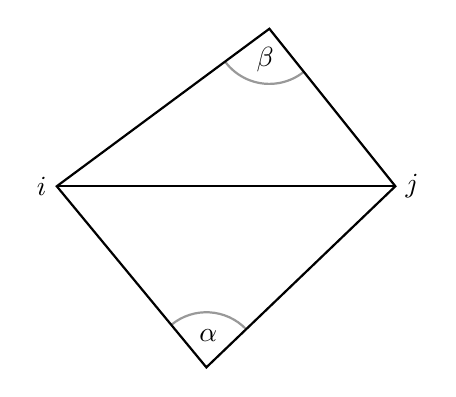
\begin{tikzpicture}[thick]
\coordinate[label=left:$i$] (O) at (-0.3,0);
\coordinate[label=right:$j$] (A) at (4,0);

\coordinate (B) at (2.4,2); % upper guy.

\coordinate (D) at (1.6,-2.3); % lower guy.

%\draw (O)--(A)--(B)--cycle;
%\draw (O)--(A)--(D)--cycle;
\draw (B)--(O)--(D)--(A)--cycle;

\draw (O)--(A);


\tkzMarkAngle[fill=gray,size=0.7cm,%
opacity=.4](O,B,A)
\tkzLabelAngle[pos = 0.4](O,B,A){$\beta$}

\tkzMarkAngle[fill=gray,size=0.7cm,%
opacity=.4](A,D,O)
\tkzLabelAngle[pos = 0.4](A,D,O){$\alpha$}


\end{tikzpicture}
\end{document}